\documentclass{beamer}
\usetheme{Madrid}
\usecolortheme{seahorse}
\usepackage[utf8]{inputenc}
\usepackage[portuguese]{babel}
\usepackage{graphicx}
\usepackage{amsmath}

\title{A Anatomia de um Motor de Busca em Larga Escala}
\subtitle{Baseado em "The Anatomy of a Large-Scale Hypertextual Web Search Engine"}
\author{Sergey Brin \and Lawrence Page}
\institute{Stanford University}
\date{1998}

\begin{document}

\begin{frame}
    \titlepage
\end{frame}

\begin{frame}{Sumário}
    \tableofcontents
\end{frame}

\section{Introdução}
\begin{frame}{Introdução}
    \begin{itemize}
        \item Desafios da recuperação de informação na Web
        \item Limitações dos índices mantidos por humanos (ex: Yahoo!)
        \item Problemas com motores de busca baseados apenas em palavras-chave
        \item Necessidade de sistemas com maior precisão
    \end{itemize}
\end{frame}

\section{Google: Objetivos de Design}
\begin{frame}{Google: Objetivos de Design}
    \begin{block}{Objetivos Principais}
        \begin{itemize}
            \item Melhorar a qualidade dos resultados de busca
            \item Desenvolvimento no âmbito acadêmico
            \item Suporte a pesquisa em larga escala
            \item Arquitetura escalável
        \end{itemize}
    \end{block}
\end{frame}

\section{Características do Sistema}
\begin{frame}{Características do Sistema}
    \begin{block}{Funcionalidades Chave}
        \begin{itemize}
            \item \textbf{PageRank}: Utiliza a estrutura de links para classificar páginas
            \item \textbf{Anchor Text}: Usa texto de links para descrever páginas de destino
        \end{itemize}
    \end{block}
\end{frame}

\subsection{PageRank}
\begin{frame}{PageRank}
    \begin{block}{Definição Matemática}
        \[ PR(A) = (1 - d) + d \left( \frac{PR(T1)}{C(T1)} + \cdots + \frac{PR(Tn)}{C(Tn)} \right) \]
        \begin{itemize}
            \item $d$: fator de amortecimento (normalmente 0.85)
            \item $C(A)$: número de links que saem da página A
        \end{itemize}
    \end{block}
    
    \begin{block}{Interpretação}
        Modelo do "navegador aleatório" que clica em links até se entediar
    \end{block}
\end{frame}

\subsection{Anchor Text}
\begin{frame}{Anchor Text}
    \begin{itemize}
        \item Texto dos links associado à página de destino
        \item Vantagens:
        \begin{itemize}
            \item Descrições mais precisas que o conteúdo da página
            \item Permite indexar documentos não-texto (imagens, programas)
            \item Expande a cobertura sem necessidade de crawler
        \end{itemize}
        \item 259 milhões de anchors indexados em 24 milhões de páginas
    \end{itemize}
  \end{frame}

\section{Arquitetura do Sistema}
\begin{frame}{Arquitetura do Google}
    \begin{center}
        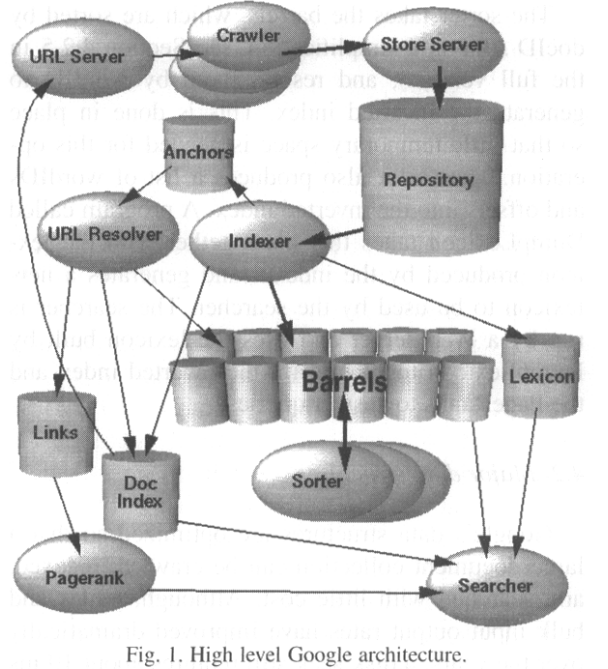
\includegraphics[height=0.8\textheight]{arquitetura.png}
    \end{center}
    \begin{tiny}
        Componentes: URLserver, Crawlers, Storeserver, Indexer, Sorter, etc.
    \end{tiny}
\end{frame}

\begin{frame}{Componentes Principais}
    \begin{itemize}
        \item \textbf{Crawlers}: Baixam páginas da Web (3 crawlers, 300 conexões cada)
        \item \textbf{Repository}: Armazena páginas comprimidas
        \item \textbf{Indexer}: Processa documentos e gera hits
        \item \textbf{Sorter}: Cria índice invertido
        \item \textbf{Searcher}: Processa consultas dos usuários
    \end{itemize}
\end{frame}

\section{Estruturas de Dados}
\begin{frame}{Estruturas de Dados Principais}
    \begin{itemize}
        \item \textbf{Repository}: HTML comprimido (53.5 GB)
        \item \textbf{Document Index}: Informações sobre cada documento
        \item \textbf{Lexicon}: Tabela hash em memória
        \item \textbf{Forward/Inverted Index}: Barris organizados por wordID/docID
        \item \textbf{Hit Lists}: Posição, fonte, capitalização (2 bytes/hit)
    \end{itemize}
\end{frame}

\section{Desempenho e Resultados}
\begin{frame}{Estatísticas de Armazenamento}
    \begin{center}
        \begin{tabular}{|l|r|}
            \hline
            \textbf{Componente} & \textbf{Tamanho} \\
            \hline
            Páginas baixadas & 147.8 GB \\
            Repository comprimido & 53.5 GB \\
            Índice invertido & 41.3 GB \\
            Lexicon & 293 MB \\
            Total & 108.7 GB \\
            \hline
        \end{tabular}
    \end{center}
\end{frame}

\begin{frame}{Estatísticas da Web}
    \begin{center}
        \begin{tabular}{|l|r|}
            \hline
            \textbf{Métrica} & \textbf{Quantidade} \\
            \hline
            Páginas baixadas & 24 milhões \\
            URLs vistos & 76.5 milhões \\
            Emails encontrados & 1.7 milhões \\
            Erros 404 & 1.6 milhões \\
            \hline
        \end{tabular}
    \end{center}
\end{frame}

\begin{frame}{Desempenho}
    \begin{itemize}
        \item Crawling: 48.5 páginas/segundo (pico)
        \item Indexação: 54 páginas/segundo
        \item Consultas: 1-10 segundos
        \item Ordenação: 24 horas (4 máquinas em paralelo)
    \end{itemize}
\end{frame}

\section{Conclusões}
\begin{frame}{Conclusões}
    \begin{block}{Contribuições}
        \begin{itemize}
            \item Motor de busca de alta qualidade
            \item Arquitetura escalável
            \item Ferramenta de pesquisa acadêmica
            \item Uso inovador de hipertexto
        \end{itemize}
    \end{block}
\end{frame}

\begin{frame}{Trabalho Futuro}
    \begin{itemize}
        \item Escalar para 100 milhões de páginas
        \item Melhorar eficiência (cache, subíndices)
        \item Atualizações inteligentes
        \item Operadores booleanos, stemming
        \item Personalização do PageRank
        \item Clusterização de resultados
    \end{itemize}
\end{frame}

\begin{frame}{Impacto}
    \begin{center}
        \Large
        Google revolucionou a busca na Web\\
        \vspace{1cm}
        \normalsize
        Combinando PageRank, anchor text e proximidade\\
        para fornecer resultados de alta qualidade
    \end{center}
\end{frame}

\begin{frame}
    \begin{center}
        \Huge Obrigado!
        \vspace{1cm}
        
        \normalsize
        Apresentação baseada no artigo:\\
        ``The Anatomy of a Large-Scale Hypertextual Web Search Engine''\\
        Sergey Brin e Lawrence Page, 1998
    \end{center}
\end{frame}

\end{document}